%%%%
\documentclass[a4paper,11pt]{article}
%%%%
%%%%
%PACKAGES______________________________________________________________________________________
\usepackage{simplewick} %Allows Wick Notation
\usepackage{slashed} %Allows feynman slash notation 
\usepackage{graphicx} % graphics, pictures, figures
\usepackage{caption}
\usepackage{subcaption}
\usepackage{verbatim} % importing numerical scripts
\usepackage{multicol, float} % placing floats in right places
\usepackage{algpseudocode} % no idea...
\usepackage[utf8]{inputenc}
\usepackage{amssymb} %needed if not using mathdesign
\usepackage{amsmath}
\usepackage[OT1]{fontenc}
\usepackage{lmodern} %gfsartemisia, times, boisik, et cetera
\usepackage{braket} %dirac notation
\usepackage[cm]{fullpage} % for fulpage style
\usepackage{bm} % boldface vectors
\usepackage{float} % placing floats
\usepackage{relsize} % for \mathlarger command
\usepackage{mathrsfs} %?
\usepackage{textgreek} % cb-greek class
\usepackage{sectsty} % for centering sections
\usepackage{textcomp } % for nr. symbol
\usepackage[usenames, dvipsnames]{color} % defining own colors
\usepackage{type1cm} % scalable fonts
\usepackage{lettrine} % larger first letter in paragraph.
\usepackage{listings} % code-snippets in the text
\usepackage{background} % used for top page text
%\usepackage{niceframe} % for old-school double frame
\usepackage{tikz} % figure config/ creation
%\usepackage{bbold}
%\usepackage{swrule} % for fancy line
%\usepackage{pdfpages} % for importing pdf

%%%%
%%%% SET-UP NEEDED FOR FURTHER PACKAGES
%%%%
\definecolor{hyperclrblue}{RGB}{30,90,125} %Definind own color ; blue
\definecolor{hyperclrorng}{RGB}{210,100,45}%Definind own color
\definecolor{hyperclrgreen}{RGB}{60,120,20}%Definind own color
\usepackage[colorlinks = true,
linkcolor = hyperclrblue,
urlcolor = blue,
citecolor = blue,
anchorcolor = blue]{hyperref} % link package
\usepackage{pgfplots} % to plot directly into latex
\pgfplotsset{compat=1.5} % needed forpgfplots
\usepackage{framed, color} % for framing/shaded box
\definecolor{shadecolor}{cmyk}{0,0,0.185,0} % color for shaded box
\usepackage{fancybox}
\usepackage[sc]{titlesec} % title package
%_______________________________________________________________________________________________
%NEW COMMANDS_________________________________________________________________________________
%\renewcommand*{\thefootnote}{$\dagger$} % creating dagger footnote
\newcommand*{\boisik}{\fontfamily{bsk}\selectfont} % change font to boisik command
\newcommand{\wf}{\text{\textpsi}} % defining wavefunctions as cbgreek class.
\newcommand{\bwf}{\text{\textPsi}} % defining Wavefunctions as cbgreek class.
\newcommand{\Q}{\hat{\text{\boisik Q}}} % defining operator-style 'Q'
\newcommand{\nlm}{\ket{n\ell m_\ell}} % defining wavefunctions as cbgreek class.
\newcommand{\nlmz}{\ket{n\ell m_\ell;0}} % defining wavefunctions as cbgreek class.
\newcommand{\nlmt}{\ket{n\ell m_\ell;t}} % defining wavefunctions as cbgreek class.
%_____________________________________________
%\numberwithin{equation}{section} %equations labeled by section
\sectionfont{\centering} % centering sections with 'sectsty'
\subsectionfont{\centering} % centering sections with 'sectsty'
\definecolor{myclr}{RGB}{190,90,20} %Definind own color
\renewcommand{\thesection}{\Roman{section}.} % Roman numerals for sections
\renewcommand{\thesubsection}{\Alph{subsection}} % Roman numerals for subsections
\titleformat{\section}{\large\scshape\centering}{\thesection}{1em}{} % Change the look of the section titles
\titleformat{\subsection}{\normalsize\centering\bfseries}{\thesubsection.}{1em}{} % Change the look of the section titles
\setlength{\columnsep}{0.7cm}
%______________________________________________________________________________________________
%%%%
%%%%_________________________________________________________________________________________
\begin{document}
%%%% TOP PAGE TEXT
{\SetBgContents{ \textit{{\small\textsc{ Ask J. Markestad, Thorbjørn V. Larsen Universitetet i Oslo. \hspace{3.5cm} \textit{\today}}}}}
\SetBgScale{1}
\SetBgColor{black}
\SetBgAngle{0}
\SetBgOpacity{1}
\SetBgPosition{current page.north east}
\SetBgVshift{-1.2cm}
\SetBgHshift{-10.5cm}
%%%% CREATING TITLE HEADER
$$\:$$
\begin{center}
	\vspace{0.2cm}%\boisik
	\fontsize{15}{15}\selectfont \textsc{ 3D Quantum Mechanical oscillator with interaction term solved with Jacobi's method}\\
	%{in}}\\
	\fontsize{13}{13}\selectfont \textsc{Fys $\textnormal{{4150}}$: Project 2}\\
	\vspace{0.4cm}
	\fontsize{12}{12}\selectfont {\textsc{ Ask J. Markestad, Thorbjoern V. Larsen }}\\
	\vspace{0.5cm}
\end{center}
%%%%
%%%%
%______________________________________________________________________________________________
%%%%
%%%%
	
%\includegraphics[scale = 0.48]{line}
\rule{\textwidth}{0.3pt}\par
		
%---------------------------------------------------------------------------------------------------------------------------------------
\begin{abstract}
	Jacobis method
\end{abstract}



		
\section*{Introduction}
		
		
		
		
\section*{Theory and Algorithms}
		\begin{equation}
\begin{pmatrix}
	2 & -1 & 0 & ... & ... & 0 \\
	-1 & 2 & -1 & 0 & ... & 0 \\
	0 & -1 & 2 & -1 & 0 & ... \\
	... & ... & ... & ... & ... & ... \\
	0 & ... & 0 & -1 & 2 & -1 \\
	0 & 0 & ... & 0 & -1 & 2 
	\end{pmatrix} \begin{pmatrix}
	u_1\\
	u_2\\
	u_3\\
	...\\
	...\\
	u_n
	\end{pmatrix} = \begin{pmatrix}
	f_1 h^2 \\
	f_2 h^2 \\
	f_3 h^2 \\
	... \\
	... \\
	f_n h^2 \\
	\end{pmatrix}
\end{equation}		




\subsection{Algorithms}

Source code and accompanying codes can be found at the git hub address:

\url{https://github.com/ajmarkestad/Fys4150/tree/master/Project2} 


\begin{lstlisting}
//general forward algorithm
for (int i=1; i<=n; i++)
	{
	b[i]=b[i]-c[i-1]*b[i-1]/b[i-1];
	f[i]=f[i]-c[i-1]*f[i-1]/b[i-1];
	}
\end{lstlisting}


Since our matrix is a tridiagonal symmetric matrix, Jacobi's method is not the best algorithm to find eigenvalues and eigenvectors. While it also works on a general dense matrix, we also wanted to test versus a standard library method that is already implemented in armadillo. This is the divide-and-conquer method\ which should scale in the general case of a dense matrix as $4n^3$ flops\cite{Divide-and-conquer}. It is rather easy to implement with the following lines
\begin{lstlisting}
mat B = A; //copy for the ARMADILLO solver
vec eigval;
mat eigvec;
eig_sym(eigval, eigvec, B);
\end{lstlisting}
It is important to note that both methods are not optimised for the tridiagonal case and are ment for dense symmetric matrices. While this might seem like a strange idea, we can use this to see how Jacobi's method performs compared to other state of the art algorithms. 





\subsection{Unit-tests}
There exist certain mathematical properties that could be exploited to make sure the program and the algorithms run correctly. Since the transformations that occur in the Jacobi's method are either orthogonal or unitary, one can see that the inner product of a given matrix will stay invariant. Under the orthogonal transformation U one has
\begin{align}
	v^{T}v = v^T U^T U v = (Uv)^T (Uv) = w^T w
\end{align}
while for a unitary transformation W and general complex v
\begin{align}
	v^\dagger v = v^\dagger W^\dagger W v = (Wv)^\dagger (Wv) = w^\dagger w
\end{align}
We see that under these transformation the inner product is conserved. We can also check whether orthogonality also is conserved. In the initial basis $\{u_i\}$ the orthogonality relation is $u_j^\dagger u_i = \delta_{ij}$. We transform as earlier
\begin{align}
	 \delta_{ij}=u_j^\dagger u_i = u_j^\dagger W^\dagger W u_i = w_j^\dagger w_i
\end{align}
which we see has the same property in the transformed system. We can use these identities to construct tests after the Jabobis method calculation, to ensure that machine error in representing numbers not will perturb the results after running a high number of iterations. We implement this as a unittest for a random, symmetric (10x10) matrix as an initial test of the algorithm and in the end of a run with the full blown set of eigenvectors. 
\begin{lstlisting}
//Orthogonality test   
for i=0 : n
        for j=0 : n
            innerproduct = dot(vector(i),vector(j))
            if ((i==j) && (abs(abs(innerproduct)-1) > pow(10,-12))) result = "bad";
            if ((i!=j) && (abs(innerproduct)>pow(10,-12))) result = "bad";
        }
    }
\end{lstlisting}
In this setting conserved is a test that the difference is smaller that a given tolerance (in our case $\epsilon = 10^{-12}$). There is also another set of tests that are useful while constructing the programs. These tests rely on simple constructed problems that are solved analytically and compared to the solutions the algorithms give. As we want to find eigenvalues and vectors, we can construct the matrix 
\begin{align}
\begin{pmatrix}
3 & \sqrt{2} \\
0 & -1 
\end{pmatrix}
, \quad \lambda_1 = -1, \quad \lambda_2 = 3, \quad v_1 = \begin{pmatrix}
-\frac{1}{2\sqrt{2}} \\
1
\end{pmatrix}, \quad v_2 = \begin{pmatrix}
1 \\
0
\end{pmatrix}
\end{align}
As a solution the program gives -1 and 3 which corresponds perfectly with the analytic solutions. To make sure the subroutines also runs, a test of the functions that finds the maximum off-diagonal element is also included in the startup tests. We initialise a 3x3 empty matrix $\hat{A}$ with the element $A_{1,2}=1$ to make sure it finds this element, with the correct column and row. For a verification that negative elements function correctly, we also test that on a similar zero-matrix with the element $A_{2,1}=-20, A_{1,2}=1$ the value -20 is picked out. 






\section*{Results}
The choise of $\rho_{max}$ and the grid size is slightly tricky as we want to make sure we extend the radius long enough to make sure the wavefunction has time to go sufficiently to zero while keeping the spatial resolution high enough not to affect the eigenvalues. From the differential equation with the interaction case it is obvious that for low $\omega$ there might be some problems in extending $\rho_{max}$ as the system naturally broadens from the weak oscillator force. In the first test we wanted to make sure we got the same results as the analytical solutions, and were interested in how far we needed to push the grid-size to get 4 digits accuracy. From the article (INSERT REFERENCE) we know that the first analytic eigenvalues for $\omega = 1$ and Columb Factor$=0$ should be 3, 7 and 11.  From an arbitrary chosen simulation of 300x300 in figure \ref{fig:test1} it is obvious that $\rho_{max}$ = 3 gives a too short size for the higher eigenvectors as these in general are pushed further out. Nevertheless we see that for the lowest eigenvalue we get an almost 3 digits correct. We could try to push this up to a higher $\rho_{max}$ but also keeping the relative size of the grids roughly the same.  After going up to n=500 and $\rho_{max}=5$ all the first 4 digits are correct as shown in figure \ref{fig:goodtest1}. We suspect that for higher eigenvalues that stretch farther out there is a need for a higher maximal size of the grid together with higher grid sizes for a given precision, and a visual inspection for a general choice of $\omega$ and Columb Factor to see that all wavefunctions to sufficiently close to zero is a fair method of choosing $\rho_{max}$ and then let the grid size be roughly $\rho_{max}*100$. 

\begin{figure}
	\centering
	\begin{subfigure}[b]{0.4\textwidth}
		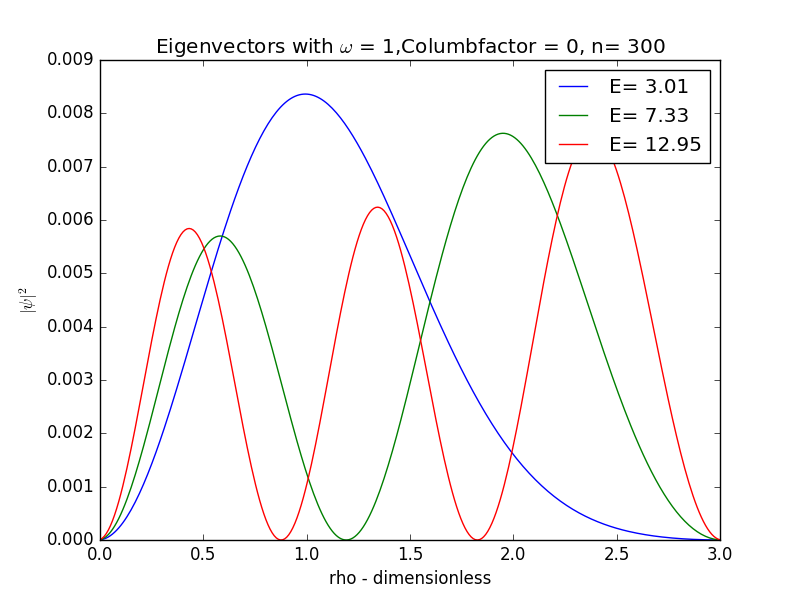
\includegraphics[scale=0.4]{ok_test1_WR=1_CF=0_C=300_rhostop=3}
		\caption{Harmonic oscillator with grid size $=300$, $rho_{max}=3$, $\omega=1$ and Columb Factor $=0$. }
		\label{fig:test1}
	\end{subfigure}
	\begin{subfigure}[b]{0.4\textwidth}
		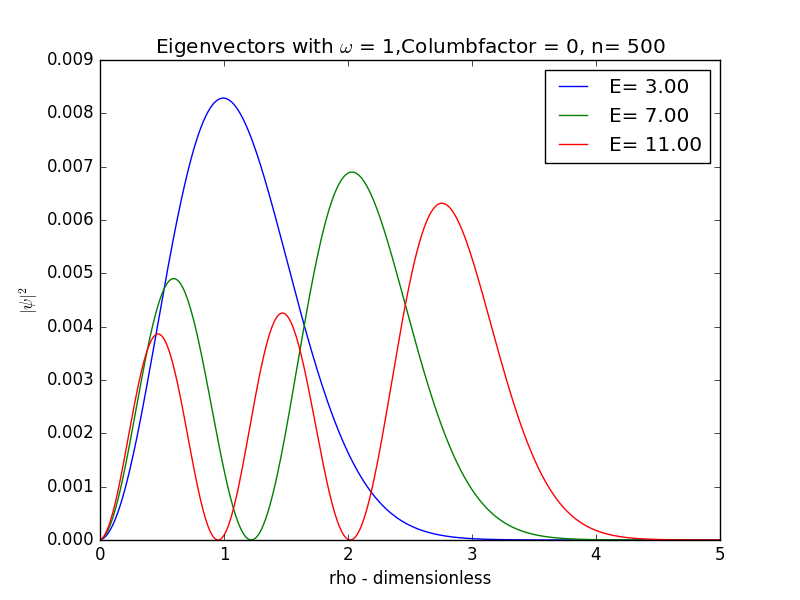
\includegraphics[scale=0.4]{ok_Project_2_Wr=1_Columb_factor=0_n=500_rho_stop=5}
		\caption{Harmonic oscillator with grid size $=500$, $rho_{max}=5$, $\omega=1$ and Columb Factor $=0$. }
		\label{fig:goodtest1}
	\end{subfigure}
\end{figure}

In the general case with a interaction term we want to see how the strength of the oscillator affects the distribution. We used the recommended values of $\omega = (0.01, 0.5, 1, 5)$. We notices that for a high omega the distribution is pushed towards lower $\rho$ values and for lower values one runs into problems as the distribution is very wide. After choosing appropriate $\rho$ and n the eigenvalues for the energy is seen in table \ref{tab:varying_omega}. As the strength of the harmonic oscillator potential increases, there is an strong increase in the energy-eigenvalues and from the plots of the distributions the electrons are restricted much closer to each other, which is no surprise. 

\begin{table}
\caption{default}
\begin{center}
\begin{tabular}{|c||c|c|c|}
\hline
Eigenvalue & $\lambda_1$ & $\lambda_2$ & $\lambda_3$ \\
\hline
\hline
$\omega=0.01$ & 0.599 & 0.968 & 1.347  \\
\hline
$\omega=0.5$ & 3.001 & 5.710 & 8.464 \\
\hline
$\omega=1$ & 4.058 & 7.910 & 11.82 \\
\hline
$\omega=5$ & 8.323 & 17.03 & 25.85 \\
\hline
\end{tabular}
\end{center}
\label{tab:varying_omega}
\end{table}%



\subsection{Scaling and flops}
To check the performance and scaling with respect to the grid size, an brute force test that runs the algorithm for different n from 50 to 1000 was performed. Then to find the scaling one approximates the total number of flops with time spend expresses this as a relation which is expected to become more precise for large n
\begin{align}
	T \propto n^{a} 
\end{align}
\begin{align}
	log_{10}(T) \approx a\cdot log_{10}(n)
	\label{eq:scaling}
\end{align}
In figure \ref{fig:scaling} one sees that there is a relation between the grid size and the number of operations. After doing a linear regression on the data with equation \ref{eq:scaling} one finds that 
\begin{align}
	T \approx n^{4.0}
\end{align}
This means that the Jacobi's method scales poorly with increasing grid size. Note that these values are expected to be hardware dependent as the number of operations per second varies with the computer, but the values are nevertheless guiding in evaluating the algorithm. The built in method of divide-and-conquer scales much better and is already faster at $n=50$. The memory requirements for both methods would also be interesting to study how Jacobi's method does with respect to this dimension as well. From the results of this scaling test we used the armadillo method for $n>200$ to increase the speed of our calculations as the Jacobi's method simply was to slow in this regieme(1 hour for 1000x1000 compared to 0.7 s is a no-brainer). 
\begin{figure}
	\centering
	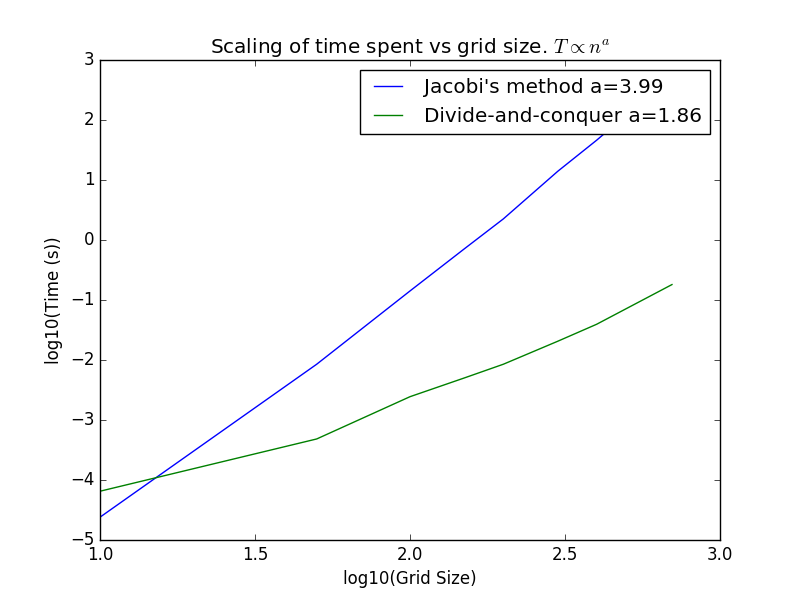
\includegraphics[scale=0.6]{Project2_scaling_time}
	\caption{Time spend on finding eigenvalues/vectors for Jacobi's method and the Divide-and-conquer method.  This data is from a run on a Macbook Pro 13' }
	\label{fig:scaling}
\end{figure}







\section*{Conclusion}
 Jacobi's method is an easy to implement method for finding eigenvalues and eigenvectors for linear algebra problems with symmetric, square matrices up to 1000x1000. Since the scaling behaviour is poor ($time \approx n^{4}$) for tridiagonal problems, is it not useful as an algorithm for matrices larger that this size. 
		
		
\begin{thebibliography}{3}
			
	\bibitem{M.Hjort-Jensen_CompFys}
	Morten Hjort-Jensen
	\emph{ Computational Physics Lecture Notes Fall 2015}
	Department of Physics, University of Oslo
	2015
	\url{https://github.com/CompPhysics/ComputationalPhysics/blob/master/doc/Lectures/lectures2015.pdf}
	
	\bibitem{Divide-and-conquer}
	Wikipedia: Divide-and-conquer method
	\url{https://en.wikipedia.org/wiki/Divide-and-conquer_eigenvalue_algorithm}
	
			
			
			
			
\end{thebibliography}
		
		
		
		
		
		
		
		
		
%__________________________________________________________________________
\end{document}